%----------------------------------------------------------------------------------------
%	PACKAGES AND THEMES
%----------------------------------------------------------------------------------------

%\documentclass[xcolor=table]{beamer}
\documentclass{beamer}
\mode<presentation> {

% The Beamer class comes with a number of default slide themes
% which change the colors and layouts of slides. Below this is a list
% of all the themes, uncomment each in turn to see what they look like.

%\usetheme{default}
%\usetheme{AnnArbor}
%\usetheme{Antibes}
%\usetheme{Bergen}
%\usetheme{Berkeley}
%\usetheme{Berlin}
%\usetheme{Boadilla}
%\usetheme{CambridgeUS}
%\usetheme{Copenhagen}
%\usetheme{Darmstadt}
%\usetheme{Dresden}
%\usetheme{Frankfurt}
%\usetheme{Goettingen}
%\usetheme{Hannover}
%\usetheme{Ilmenau}
%\usetheme{JuanLesPins}
%\usetheme{Luebeck}
\usetheme{Madrid}
%\usetheme{Malmoe}
%\usetheme{Marburg}
%\usetheme{Montpellier}
%\usetheme{PaloAlto}
%\usetheme{Pittsburgh}
%\usetheme{Rochester}
%\usetheme{Singapore}
%\usetheme{Szeged}
%\usetheme{Warsaw}

% As well as themes, the Beamer class has a number of color themes
% for any slide theme. Uncomment each of these in turn to see how it
% changes the colors of your current slide theme.

%\usecolortheme{albatross}
%\usecolortheme{beaver}
%\usecolortheme{beetle}
%\usecolortheme{crane}
%\usecolortheme{dolphin}
%\usecolortheme{dove}
%\usecolortheme{fly}
%\usecolortheme{lily}
%\usecolortheme{orchid}
%\usecolortheme{rose}
%\usecolortheme{seagull}
%\usecolortheme{seahorse}
%\usecolortheme{whale}
%\usecolortheme{wolverine}

%\setbeamertemplate{footline} % To remove the footer line in all slides uncomment this line
%\setbeamertemplate{footline}[page number] % To replace the footer line in all slides with a simple slide count uncomment this line

\setbeamertemplate{navigation symbols}{} % To remove the navigation symbols from the bottom of all slides uncomment this line
}
\usepackage{tcolorbox}
\usepackage{graphicx} % Allows including images
\usepackage{booktabs} % Allows the use of \toprule, \midrule and \bottomrule in tables
\usepackage[utf8]{inputenc}
\usepackage{longtable}
\usepackage{lineno,hyperref}
\modulolinenumbers[5]
\usepackage{tablefootnote}
\usepackage{threeparttable}
\usepackage{adjustbox}
\usepackage{caption}
\usepackage{bibentry}
%\captionsetup{skip=-5pt}

%----------------------------------------------------------------------------------------
%	TITLE PAGE
%----------------------------------------------------------------------------------------

\title[overview]{Cancer Survival Statistics: an Overview} % The short title appears at the bottom of every slide, the full title is only on the title page

\author{Yuliya Leontyeva, Enoch Chen} % Your name
\institute[MEB] % Your institution as it will appear on the bottom of every slide, may be shorthand to save space
{
MEB, KI Stockholm \\ % Your institution for the title page
\medskip
}
\date{February 2, 2021} % Date, can be changed to a custom date
\titlegraphic{
\includegraphics[height=1.5cm]{logo.png}\hspace*{-9cm}}

\begin{document}

\begin{frame}
\titlepage % Print the title page as the first slide
\end{frame}

\begin{frame}
\frametitle{Cancer Survival Statistics: an Overview} % Table of contents slide, comment this block out to remove it
\textbf{Reasoning}

\begin{enumerate}
    \item Usage of the same concepts
    \item Three advanced seminars so far:
    \begin{itemize}
        \item Does the choice of timescale influence the CIF estimates in a competing risks setting? Correspondence of competing risks and relative survival by Nikolaos Skourlis
        \item Modelling multiple time-scales using flexible parametric models by Nurgul Batyrbekova
        \item Making life tables using multiple time-scale flexible parametric models by Enoch Yi Tung Chen
    \end{itemize}
\end{enumerate}
\end{frame}

%------------------------------------





\begin{frame}
\frametitle{Overview} % Table of contents slide, comment this block out to remove it
\tableofcontents % Throughout your presentation, if you choose to use \section{} and \subsection{} commands, these will automatically be printed on this slide as an overview of your presentation
\end{frame}

%----------------------------------------------------------------------------------------
%	PRESENTATION SLIDES
%---------------------------------------------------------------------------------%
\section{Introduction}
\begin{frame}
\frametitle{Introduction}
\begin{itemize}
\item Registry data
\item Talk based on but not limited to Eloranta S et al. 2020. Cancer survival statistics for patients and healthcare professionals – a tutorial of real-world data analysis.
\end{itemize}


\textbf{Advantages over clinical trials:}
 \begin{itemize}
 \item Price and time (clinical trials are more expensive and take much more time)
 \item Cohort of all patients (clinical trials with inclusion/exclusion criteria)
 \item Possible to study long effect or side effect of the treatment 
 \item Long follow-up 
 \item Linkage between different cohorts, especially in Sweden
 \end{itemize}
\end{frame}
%----------------------------------------------------------------------------------------
\section{Overview of measures and frameworks}
\begin{frame}{Overview of approaches \footnote{Summarised from Dickman2015 (Estimating and modeling relative survival)}}

\begin{figure}
    \centering
    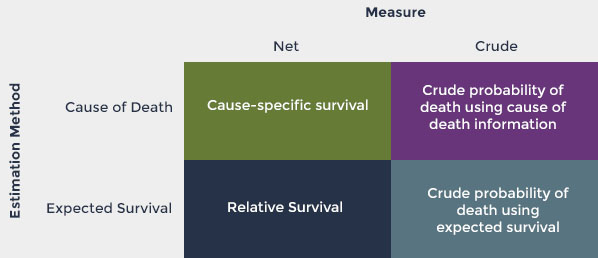
\includegraphics[scale=0.35]{survival_table.jpg}
    \caption{Measures of Cancer Survival. Figure downloaded from National Cancer Institute: https://surveillance.cancer.gov/survival/measures.html}
    \label{fig:my_label}
\end{figure}
\vspace{-20pt}
\begin{itemize}
    \item Crude survival (measure)

    \begin{itemize}
        \item Cause-specific framework
        \item Relative survival framework
    \end{itemize}
    
    \item Net survival (measure)
      \begin{itemize}
        \item Cause-specific framework
        \item Relative survival framework
    \end{itemize}
\end{itemize}

\end{frame}

\begin{frame}{\secname}
\textbf{Choose a measure based on:} \\
The purpose of the study: 
\begin{itemize}
    \item Crude survival \begin{itemize}
        \item Presence of dying from other causes rather than only the disease of interest.
        \item Clinical decisions for a specific patient
    \end{itemize}
    \item Net survival 
    \begin{itemize}
        \item hypothetical world, absence of dying from other causes
        \item comparisons over time or groups (countries)
            \end{itemize}
\end{itemize}
\end{frame}

\begin{frame}{\secname}

  \begin{figure}
    \centering
    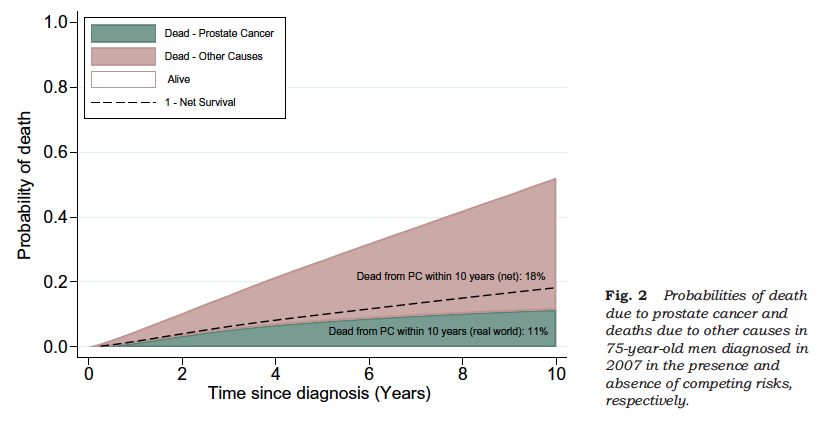
\includegraphics[scale=0.4]{stack.png}
    \caption{Eloranta2020. Shaded areas: considering competing risks (real world); dashed line: patients can only die from the disease of interest (hypothetical world)}
    \label{fig:my_label}
\end{figure}

\end{frame}
%----------------------------------------------------------------------------------------
%----------------------------------------------------------------------------------------
\begin{frame}{\secname}
\textbf{Choose framework based on:} \\
\noindent \textcolor{gray}{\textbf{(For sure, your research question of interest)}}

\noindent \textbf{Availability of cause of event info:}

\begin{itemize}
    \item Cause-specific framework - the cause of event of interest is \textbf{known} and accurate
    \item Relative survival framework - the cause of event of interest is \textbf{unknown} or not reliable (\textbf{preferable})
\end{itemize}

\end{frame}



\section{Cause-specific framework}
\begin{frame}
\frametitle{Cause-specific framework}
%----------------------------------------------------------------------------------------

\begin{itemize}
\item Advantage: It requires the cause of the event. \begin{itemize}
    \item Cause-specific hazard $\rightarrow$ cumulative incidence function (probability of patients that have died from cause $K$ at time $t$)\footnote{Hincliffe2013. Flexible parametric modelling of cause-specific hazards to estimate cumulative incidence functions.}
    \item Multi-state settings
\end{itemize}

\item Disadvantage: It requires the cause of the event.
\begin{itemize}
    \item The cause of death info might not be complete.
\end{itemize}
\end{itemize}
\end{frame}

\begin{frame}{Cause-specific framework}
\begin{figure}
    \centering
    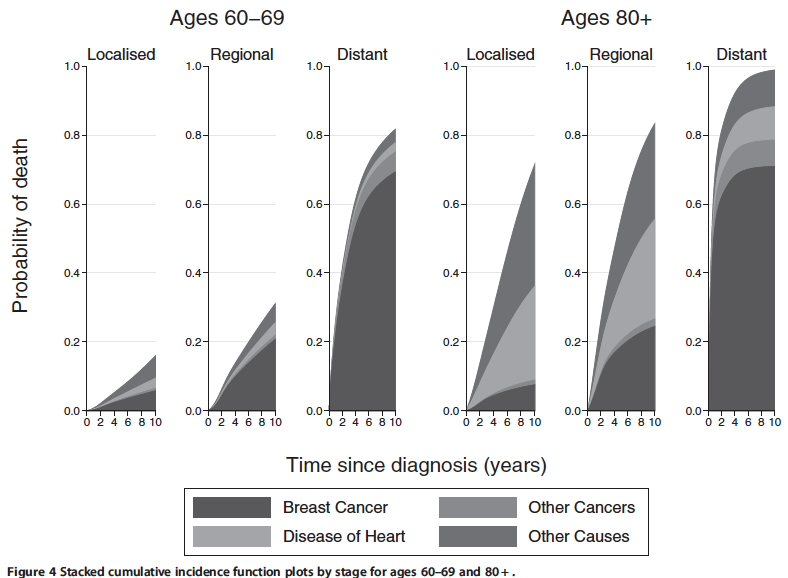
\includegraphics[scale=0.3]{compete.png}
    \caption{Hinchliffe2013. Modeling cause-specific hazards and transform them to cumulative incidence functions.}
    \label{fig:my_label}
\end{figure}
    
\end{frame}
%%%
\begin{frame}
\frametitle{Cause-specific framework}
\begin{itemize}
\item Measure crude survival: competing risks settings, patients might die from other causes than the disease under study.

\item Measure net survival: censor all the other causes 

\end{itemize}
\begin{figure}
    \centering
    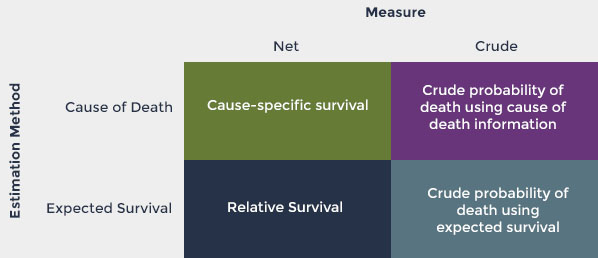
\includegraphics[scale=0.3]{survival_table.jpg}
    \caption{Measures of Cancer Survival. Figure downloaded from NCI}
    \label{fig:my_label}
\end{figure}
\end{frame}
%----------------------------------------------------------------------------------------
\begin{frame}
\frametitle{Relative survival framework}

\begin{itemize}
\item Advantage: It does not require the cause of the event $\rightarrow$ can incorporate both direct and indirect causes


\item Relative survival is estimated as comparison of survival in the cohort with survival in the general population $\rightarrow$ {need of life tables} 

\item The Human Mortality Database \footnote{https://www.mortality.org/}
\end{itemize}
\end{frame}

\begin{frame}
\frametitle{Net survival}
Assumptions to interpret as Net survival
\begin{itemize}
    \item \textbf{Exchangeability} If a cancer patient did not have cancer, he/she would have the same probability to survive as a similar person in the general population
    
    \item \textbf{Conditional independence} between cancer deaths and other causes of death 
\end{itemize}

\section{Relative survival framework}
\end{frame}

\begin{frame}
\frametitle{\small{Net survival in cause-specific and relative survival framework}}
\begin{figure}
\centering
    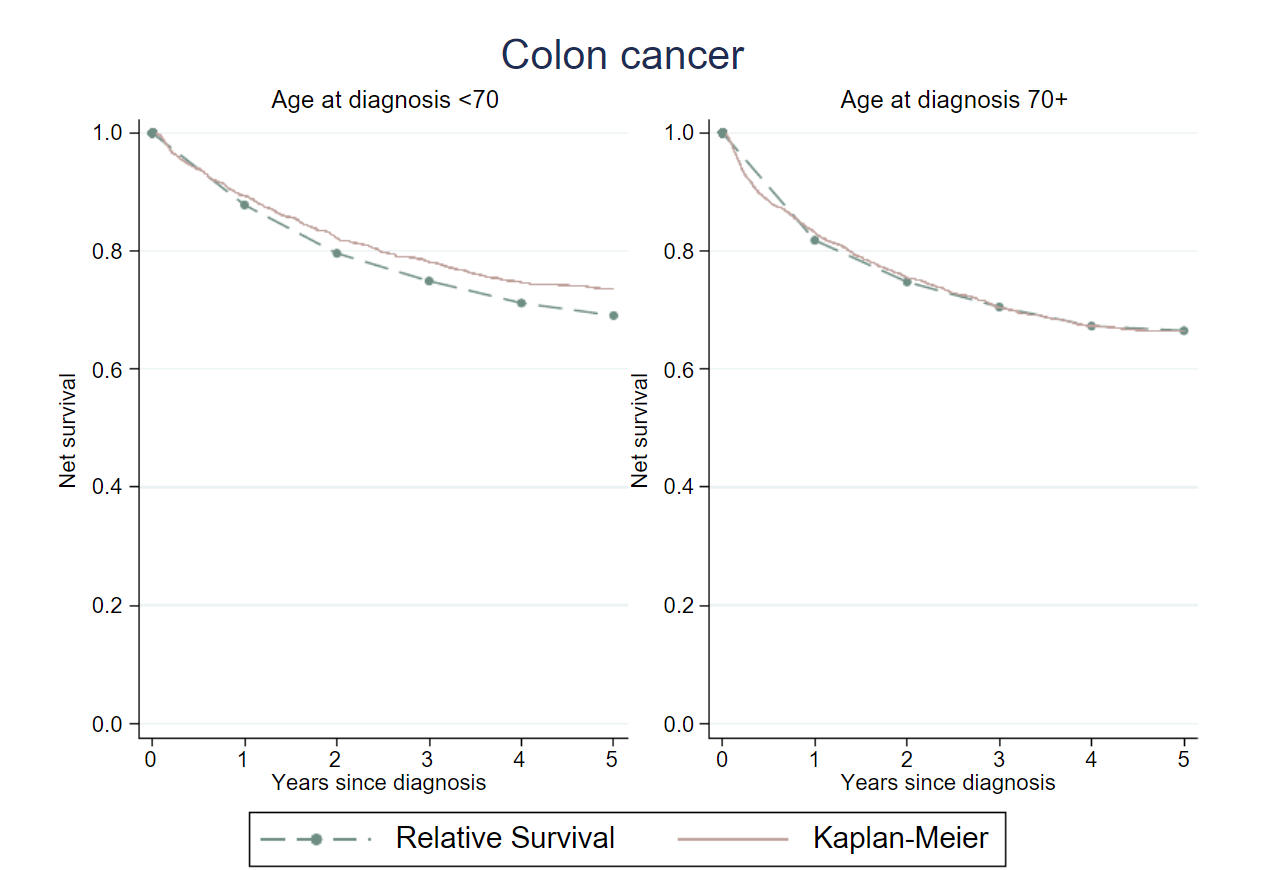
\includegraphics[scale = 0.3]{pic2.png}
\caption{Eloranta, S.et al Cancer survival statistics for patients and healthcare professionals – a tutorial of real-world data analysis}
\label{fig1}
\end{figure}
\end{frame}

\begin{frame}
\frametitle{Crude survival}
\begin{figure}
    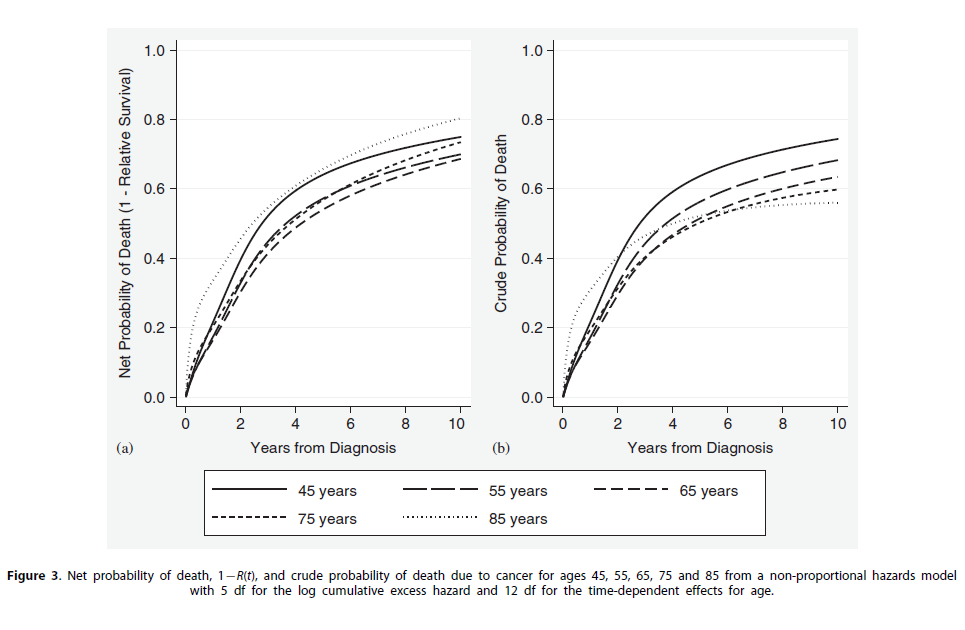
\includegraphics[scale = 0.4]{pic1.png}
\caption{Lambert, P. et al Estimating the crude probability of death due to cancer and other causes using relative survival models}
\label{fig2}
\end{figure}
\end{frame}

%----------------------------------------------------------------------------------------
\begin{frame}{Map of previous talks}
\textbf{What measure? What framework?}
\begin{itemize}
\item    Nick: Does the choice of timescale influence the CIF estimates in a competing risks setting? 
\item     Nurgul: Modelling multiple time-scales using flexible parametric models
\item     Enoch: Making life tables using multiple time-scale flexible parametric models.
\item    \textcolor{gray}{Welcome to sign up the upcoming presentations!!}
\end{itemize}  

\end{frame}

\begin{frame}{Map of previous talks}
\textbf{What measure? What framework?}

\begin{itemize}
\item    Nick: Does the choice of timescale influence the CIF estimates in a competing risks setting? \textbf{Crude survival measure - cause-specific survival framework}
\item     Nurgul: Modelling multiple time-scales using flexible parametric models \textbf{Net survival measure - cause-specific framework}
\item     Enoch: Making life tables using multiple time-scale flexible parametric models. \textbf{Net survival measure - relative survival framework}
\item    \textcolor{gray}{Welcome to sign up the upcoming presentations!!}
\end{itemize}  
\end{frame}

\section{Discussion}
\begin{frame}
\frametitle{Discussion}
\begin{enumerate}
\item What is the purpose of net survival/crude survival?
\item If you want to estimate fertility rate, which framework should be use? 
\item What is missing in the interpretation of the survival from Figure on the right \ref{fig1}: 5 years after the diagnosis 66\% of elderly men would still be alive.
\item The net probability of death underestimates / overestimates real-world probability of death from cancer.


    
\end{enumerate}
\end{frame}
%----------------------------------------------------------------------------------------


%%-----

\begin{frame}
\frametitle{References}
\footnotesize{
\begin{thebibliography}{99} % Beamer does not support BibTeX so references must be nserted manually as below
\bibitem[Eloranta, S., 2021]{p1} Eloranta, S. and Smedby, K. E. and Dickman, P. W. and Andersson, T. M. (2021)
\newblock Cancer survival statistics for patients and healthcare professionals – a tutorial of real-world data analysis
\newblock \emph{Journal of Internal Medicine} 289(1), 12 -- 28.
\bibitem[Lambert, P., 2010]{p2} Lambert, P. C.,Dickman, P. W.,Nelson, C. P.,Royston (2010)
\newblock Estimating the crude probability of death due to cancer and other causes using relative survival models
\newblock \emph{StatMed} 29(7-8), 885 -- 95.

\end{thebibliography}
}
\end{frame}


%----------------------------------------------------------------------------------------
\end{document} 


